% Research Paper for GECCO 2015
% by Nic McPhee, Kirbie Dramdahl, and David Donatucci

\documentclass{sig-alternate}

\usepackage{times}
\usepackage{url}
\usepackage{todonotes}
\sloppy

\setlength{\parindent}{0.5cm} 

\newcommand{\citep}[1]{\cite{#1}}

%\DeclareGraphicsRule{.tif}{png}{.png}{`convert #1 `dirname #1`/`basename #1 .tif`.png}

\begin{document}

\conferenceinfo{GECCO'16,} {July 20-24, 2016, Denver, CO, USA.}
\CopyrightYear{2016}
\crdata{TBA}
\clubpenalty=10000
\widowpenalty = 10000
    
\title{Visualizing genetic programming ancestries using graph databases}

%\numberofauthors{4}
%\author{
%\alignauthor
%Nicholas Freitag McPhee\\
%	\affaddr{Division of Science and Mathematics}\\
%	\affaddr{University of Minnesota, Morris}\\
%	\affaddr{Morris, MN USA-56267}\\
%	\email{mcphee@morris.umn.edu}
%\alignauthor
%Maggie M. Casale\\
%	\affaddr{Division of Science and Mathematics}\\
%	\affaddr{University of Minnesota, Morris}\\
%	\affaddr{Morris, MN USA-56267}\\
%	\email{casal033@morris.umn.edu}
%\alignauthor
%Thomas Helmuth\\
%	\affaddr{Computer Science Department}\\
%	\affaddr{Washington and Lee University}\\
%	\affaddr{Lexington, VA USA-24450}\\
%	\email{helmutht@wlu.edu}
%\alignauthor
%Lee Spector\\
%	\affaddr{Cognitive Science}\\
%	\affaddr{Hampshire College}\\
%	\affaddr{Amherst, MA USA-01002}\\
%	\email{lspector@hampshire.edu}
%}
%
\maketitle

\begin{abstract}

\textbf{We are submitting this in the hopes of it being a \textit{poster} and not a paper. There's just not a separate mechanism for submitting specifically for posters. Thanks.}

Previous work has demonstrated the utility of graph databases as a tool for collecting and analyzing ancestry in evolutionary computation runs. That work focused on sections of individual runs, whereas this poster illustrates the application of these ideas on the entirety of large runs (up to one million individuals) and combinations of multiple runs.

This will include a graph showing \emph{all} the ancestors of successful individuals from a variety of stack-based genetic programming runs on software synthesis problems. We will demonstrate how these graphs can highlight critical moments in the evolutionary process, and use them to compare the dynamics when using different evolutionary tools, such as different selection mechanisms or representations.

\end{abstract}

\section{Introduction}
\label{sec:introduction}

Typical reporting of genetic programming and evolutionary computation results is usually limited to aggregate statistics such as mean best fitness or percentage of successful runs. This fails to convey, however, the complex dynamics of such evolutionary systems and obscures or omits potentially valuable information about \emph{why} the runs behaved as they did~\cite{McPhee:2015:GPTP}.

In this poster we illustrate the use of graph database tools as a means of collecting and analyzing ancestry data from genetic programming runs. We use Titan graph database\footnote{\url{http://thinkaurelius.github.io/titan/}} along with the Gremlin shell and the Tinkerpop query tools\footnote{\url{https://tinkerpop.incubator.apache.org/}} to store the parent-child relationships in genetic programmings, as well as extract the ancestry trees of specified individuals. We then visualize these subgraphs using the Graphviz \texttt{dot} graph layout tool\footnote{\url{http://www.graphviz.org/}}.

\section{Example: Success vs. failure}
\label{sec:examples}

We  illustrate these ideas by extracting and plotting the ancestors final generation individuals in both a successful and an unsuccessful run of the replace-space-with-newline software synthesis problem~\cite{Helmuth:2015:GECCO,Helmuth:2015:dissertation} using lexicase selection~\cite{Helmuth:2014:ieeeTEC}. For example, Figure~\ref{fig:success} allows us to compare a successful and an unsuccessful run in Figure~\ref{fig:fail}. The successful run shows all the ancestors of that run's winners (i.e., individuals with total error 0); the unsuccessful run shows the ancestors of all individuals in the final generation. The unsuccessful run was capped at 300 generations; the successful run found a solution at generation 129.

In these figures generations run from the initial random population at the top to the final generation at the bottom, one generation per row. Each ancestor individual is represented as a rectangle whose width is proportional to the number of selections that individual received and whose height is proportional to the number of its offspring that were individuals included in the ancestry graph. The ratio of width to number of selections is $\frac{1}{5}$ the ratio of height to number of ancestral children to keep the graph from getting too wide. The color of an individual is determined by its total error; 0 total error is bright green, moving through blues to bright red, which represents total error of 10,000 or greater. A directed edge in the graph indicates a parent-child relation, with the edge going from the parent down to the child. A child with only a single incoming edge is the result of a mutation operator and children with two incoming edges are the result of a recombination; see~\cite{Helmuth:2015:dissertation,Spector:2013:GPTP} for additional details.

Both Figures~\ref{fig:success} and~\ref{fig:fail} illustrate a common pattern in the early generations where there a substantial number of highly selected individuals (very wide individuals), presumably because most randomly generated individuals in the first generation perform poorly (evidenced by the prevalence of red and pink). After several generations, however, the population gains competence (as evidenced by more purple and dark blue) and there are fewer instances where a single individual receives a very high proportion of the selection events, leading to mostly small rectangles representing individuals.

\begin{figure}[t]
\centering
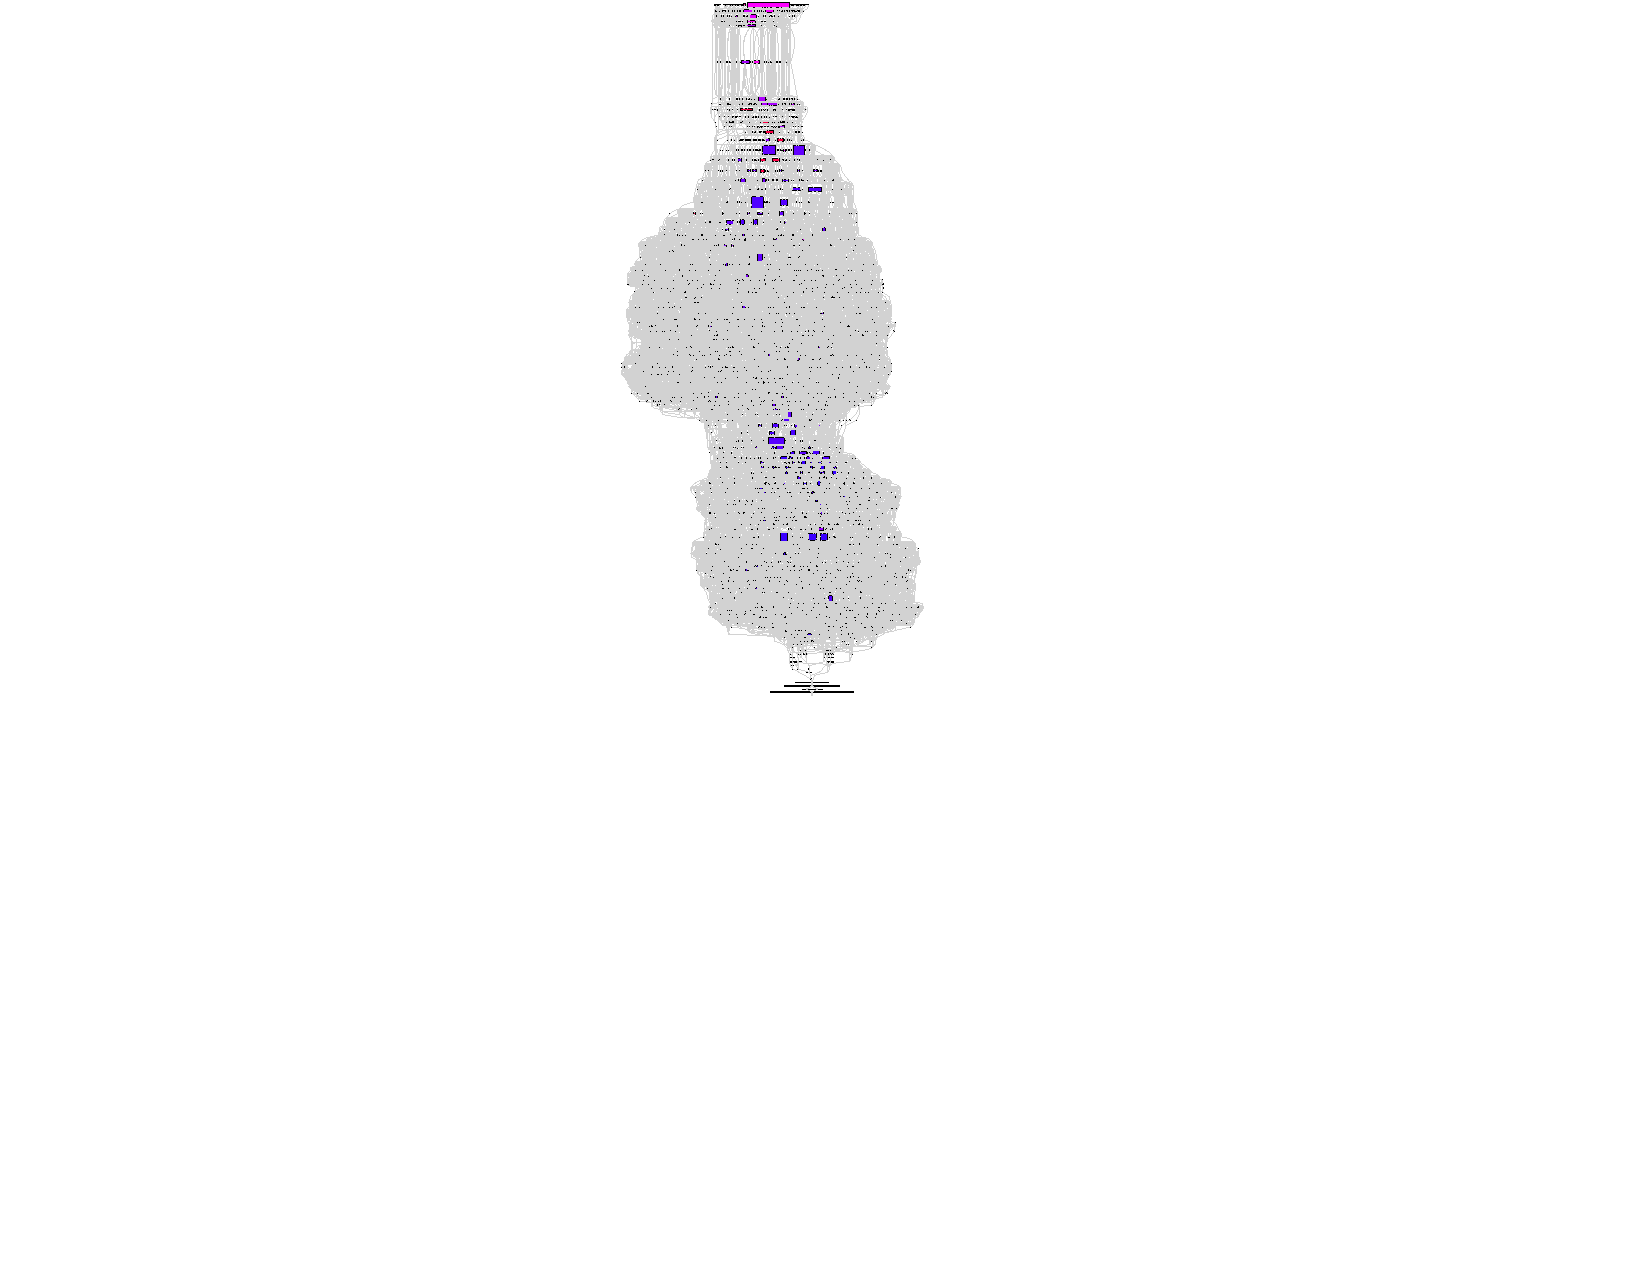
\includegraphics[height=0.5 \textheight]{../Figures/output_success.pdf}
\caption{Ancestry tree for a successful run of the replace-space-with-newline problem using lexicase selection.}
\label{fig:success}
\end{figure}

\begin{figure}[p]
\centering
\includegraphics[height=0.91 \textheight]{../Figures/output_fail.pdf}
\caption{Ancestry tree for an unsuccessful run of the replace-space-with-newline problem using lexicase selection. }
\label{fig:fail}
\end{figure}


\todo[inline]{Pull actually numbers of selections to augment the super fuzzy color references below.}

After that initial phase, the dynamics in the unsuccessful run (Figure~\ref{fig:fail}) become very ``static'', with the width of the graph (essentially the number of ancestors in each generation) remaining roughly constant with no highly selected (i.e., wide) individuals. The colors also indicate that the total error is not improving substantially over time, remaining mostly between pink and purple.

In the successful run (Figure~\ref{fig:success}), however, there are clear changes in the dynamics over time. After the initial ``settling out'', the best individual is able to correctly solve 124 of the 200 test cases for replace-space-with-newline. There is then a ``narrowing'' of the graph after about 60 generations, with several highly selected (i.e., wide) individuals dominating the ancestry there. This narrowing represents an important ``discovery'' which leads to individuals that have zero error on an additional 9\% (18) of the test cases. The graph widens out again after that, but there are still some highly selected individuals around generation 90 until the rapid convergence on the solution in the final generations.




\bibliographystyle{abbrv}
\bibliography{GECCO_2016}

\end{document}